\section{Durchführung}
\label{sec:Durchführung}

\subsection{Versuchsaufbau}
\label{sec:Versuchsaufbau}
%\begin{figure}
%	\centering
%	\caption{Schematische Darstellung des Versuchsaufbaus \cite{anleitung}.}
%	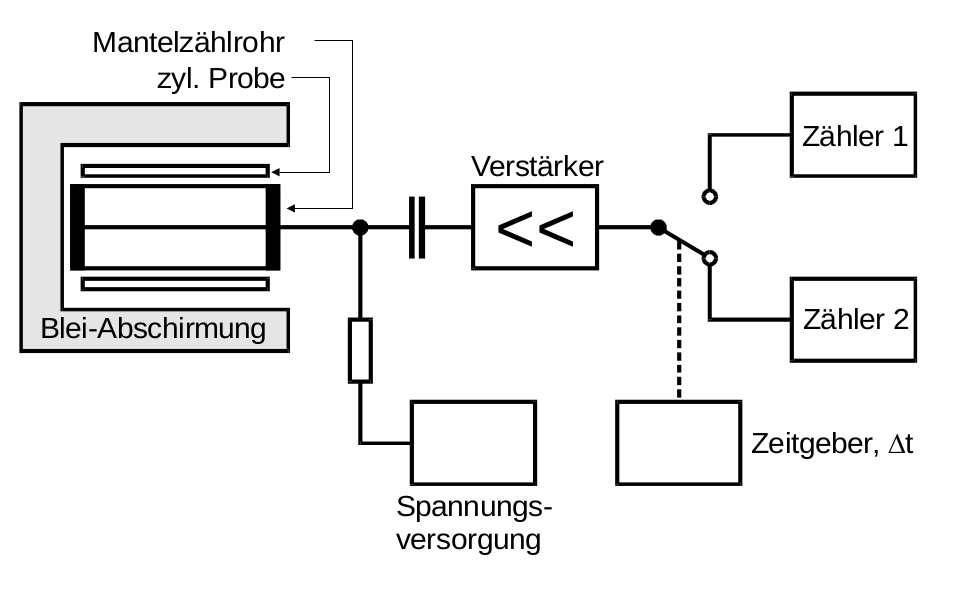
\includegraphics{Bilder/aufbau.png}
%	\label{fig:aufbau}
%\end{figure}
%
%\begin{figure}
%	\centering
%	\caption{Schematische Darstellung der Quelle zur Erzeugung radioaktiven Isotopen \cite{anleitung}.}
%	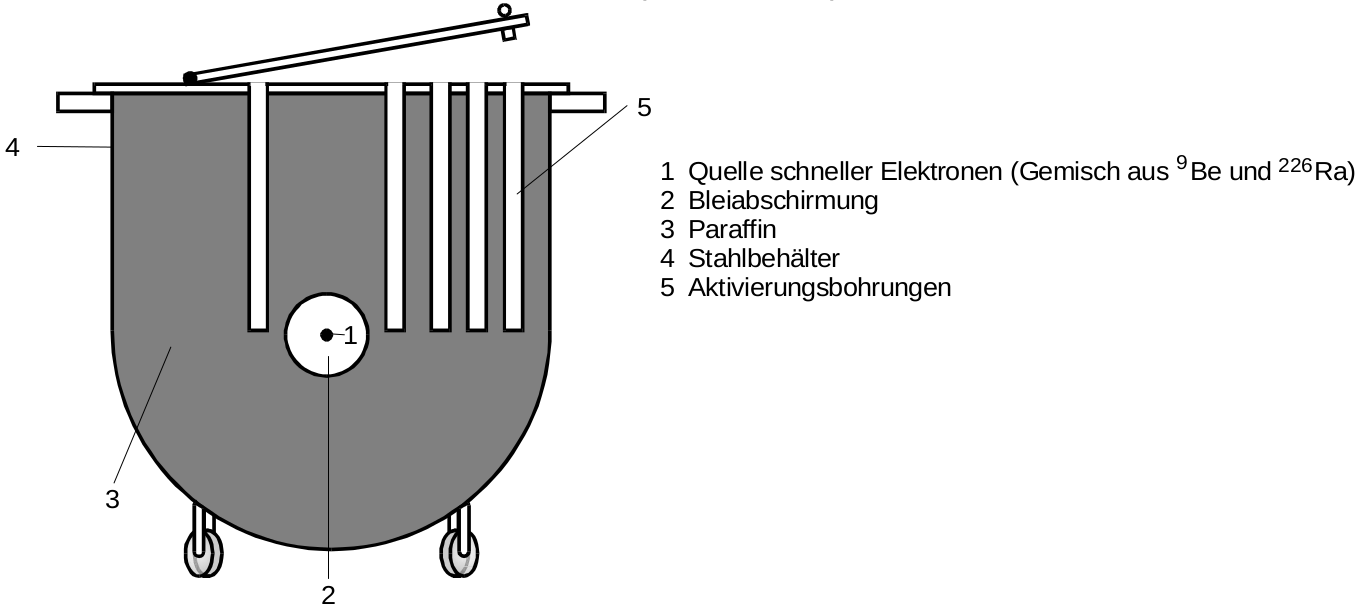
\includegraphics{content/toepfchen.png}
%	\label{fig:kochen}
%\end{figure}
%
Der Versuchsaufbau -- wie in Abbildung \ref{fig:aufbau} dargestellt -- besteht im Wesentlichen 
aus einem zerfallenden radioaktiven Isotop und einem Geiger-Müller-Zählrohr, welches die 
zerfallenden Kerne misst.
Das Geiger-Müller-Zählrohr ist entspricht einer mit Gas gefüllten Röhre. Trifft ein $\beta$-
oder $\gamma$- Teilchen auf ein Gasteilchen wird dieses ionisiert und kann aufgrund einer
anliegenden Spannung an der Röhre gemessen werden.
Dabei werden die gemessenen Zerfälle pro Messzeitintervall, welches am Zeitgeber einstellbar 
ist, an den Zählern 1 und 2 angezeigt. Nach jedem Messvorgang wird der Zähler umgeschaltet und 
der vorherige Wert auf dem aktuellen Zähler wird überschrieben. Der Versuchsaufbau ist mit
einer Blei-Abschirmung ausgestattet um die radioaktive Strahlung abzuschirmen.

Zur Erzeugung der radioaktiven Isotope wird das Objekt in Abbildung \ref{fig:kochen} verwendet.
Hierbei werden stabile Kerne mit niederenergetischen Neutronen beschossen. 
Da die Neutronen ihre Energie durch elastische Stöße an die Kerne übergeben und die maximale
Energie bei gleichen Massen der Stoßpartner erreicht wird, werden die Neutronen in einem 
Paraffinmantel gebremst, bis sie die optimale Energie besitzen.


\subsection{Versuchsbeschreibung}
\label{sec:Versuchsbeschreibung}
Vor jeder Messung wird eine Leerlaufmessung -- Nullmessung -- ohne radioaktives Isotop
durchgeführt, bei der die 
nicht zu vernachlässigenden Zerfälle der Störquellen aufgenommen werden. Diese Messung wird mit
einem Messzeitintervall von $\Delta t = \SI{900}{\second}$ durchgeführt. Die aufgenommenen 
Zerfälle bei der Nullmessung werden -- angepasst auf das Messzeitintervall -- von den 
aufgenommenen Zerfällen mit einem radioaktiven Isotop abgezogen, um den Fehler zu verringern.

Daraufhin wird der Zerfall von $^{116}$In gemessen. Hierbei werden 15 Messwerte bei einem 
Messzeitintervall von jeweils $\Delta t = \SI{240}{\second}$ aufgenommen. 

Zuletzt wird der Zerfall von dem instabilen Isotopengemisch $^{108}$Ag und $^{110}$Ag gemessen.
Diese Messung wird über einen Zeitraum von $\SI{15}{\minute}$ durchgeführt, wobei alle
$\Delta t = \SI{15}{\second}$ ein Wert notiert wird.
